\textbf{\underline{OZ 7 - Inductantie - Oefening 1:}}
\vspace{0.5cm}

Bepaal voor de toroïde de energiedichtheid in het magnetisch veld in
functie van $r$ waarbij $r_1 < r < r_2$. Integreer dit over het volume om de totale energie
opgeslagen in de toroïde te vinden. De toroïde bevat $N$ windingen en draagt een
stroom $I$.

\begin{center}
    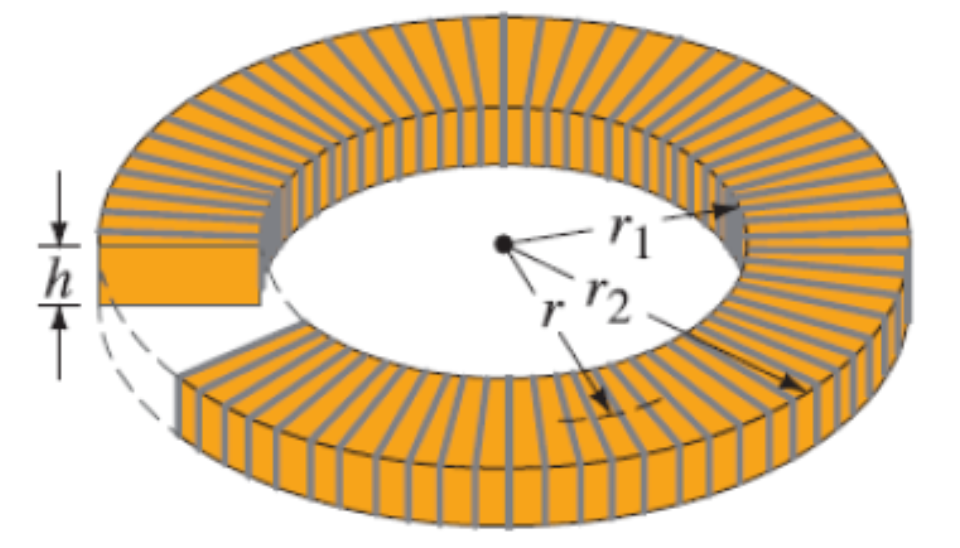
\includegraphics[scale = 0.3]{oz07/resources/Oz7Oef1.png}
\end{center}

\begin{description}[labelwidth=1.5cm, leftmargin=!]
    \item[Geg. :] $N$, $I$, $r_1 < r < r_2$
    \item[Gevr. :] $u_B$ ? 
    \item[Opl. :]
    De energiedichtheid is gegeven door $u_B = \frac{1}{2} \frac{B^2}{\mu_0}$, dus
    \begin{equation*}
        u_B(r) = \frac{\mu_0 N^2 I^2}{8\pi^2 r^2}.
    \end{equation*}
    waarover we kunnen integreren om de totale potentiele energie te vinden:
    \begin{align*}
        U_B 
            &= \int_{r_1}^{r_2} u_B(r) dV \\
            &= \int_{r_1}^{r_2} \frac{\mu_0 N^2 I^2}{8\pi^2 r^2} 2\pi r h dr \\
            &= \frac{\mu_0 N^2 I^2 h}{4\pi} \ln \left(\frac{r_2}{r_1}\right).
    \end{align*}

    \vspace{0.3cm}
    \textbf{Opmerking:} 
        Je kan de energiedichtheid ook afleiden door 
        \begin{equation*}
            u_B = \frac{dU_B}{dV}
        \end{equation*} 
        waarbij $U_B$ de energie opgeslagen in het magnetisch veld is en $V$ het volume van de toroïde. We berekenen het magnetisch veld binnen de torus
        \begin{equation*}
            \oint \vec{B} \cdot d\vec{\ell} = \mu_0 I
        \end{equation*}
        waaruit trivialiter volgt dat:
        \begin{equation*}
            B = \frac{\mu_0 N I}{2\pi r}.
        \end{equation*}  
        We hebben ook de zelfinductie nodig van de toroïde, deze is gegeven door:
        \begin{align*}
            L 
                &= \frac{N}{I} \Phi_B \\
                &= \frac{N}{I} \int_{r_1}^{r_2} \frac{\mu_0 N I h }{2\pi r} dr \\
                &= \frac{\mu_0 N^2 h}{2\pi} \ln \left(\frac{r_2}{r_1}\right).
        \end{align*}
        De energie opgeslagen in het magnetisch veld is gegeven door
        \begin{align*}
            U_B &= \frac{1}{2}LI^2 = \frac{\mu_0 N^2  I^2 h}{4\pi} \ln \left(\frac{r_2}{r_1}\right) \\
        \intertext{met energiedichtheid}
            u_B &= \frac{dU_B}{dV} = \frac{\mu_0 N^2  I^2 h}{8\pi^2r^2}.
        \end{align*}
        % met $L$ de zelfinductie van de toroïde. De energiedichtheid is dan:
        % \begin{equation*}
        %     u_B = \frac{U_B}{V} = = \frac{\mu_0 N^2  I^2 h}{4\pi^2 (r_2^2 - r_1^2)} \ln \left(\frac{r_2}{r_1}\right)
        % \end{equation*}

\end{description}

\vspace{1cm}